\chapter{Summary, Formula Sheet and Glossary}
\label{ch:summary}

\section{The whole chapter in one picture}

\begin{center}
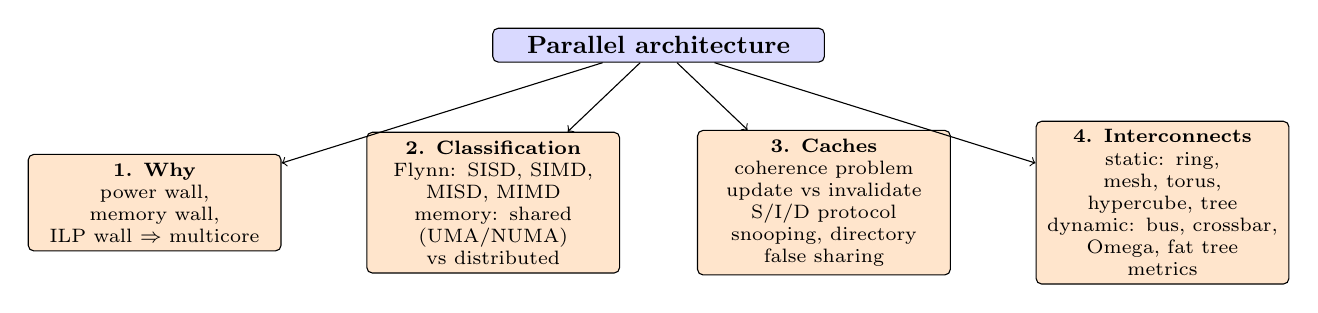
\begin{tikzpicture}[bx/.style={draw,rounded corners=2pt,fill=#1,font=\scriptsize,align=center,inner sep=3pt,text width=3.0cm}]
  \node[bx=blue!15,text width=4cm,font=\small\bfseries] (root) at (0,0) {Parallel architecture};
  \node[bx=orange!20] (a) at (-6.4,-2.0) {\textbf{1. Why}\\power wall, memory wall,\\ILP wall $\Rightarrow$ multicore};
  \node[bx=orange!20] (b) at (-2.1,-2.0) {\textbf{2. Classification}\\Flynn: SISD, SIMD, MISD, MIMD\\memory: shared (UMA/NUMA)\\vs distributed};
  \node[bx=orange!20] (c) at (2.1,-2.0)  {\textbf{3. Caches}\\coherence problem\\update vs invalidate\\S/I/D protocol\\snooping, directory\\false sharing};
  \node[bx=orange!20] (d) at (6.4,-2.0)  {\textbf{4. Interconnects}\\static: ring, mesh, torus,\\hypercube, tree\\dynamic: bus, crossbar,\\Omega, fat tree\\metrics};
  \foreach \n in {a,b,c,d} \draw[->] (root) -- (\n);
\end{tikzpicture}
\end{center}

\begin{keyidea}
Hardware designers give us parallelism because they can no longer give us speed (Chapter~1). Machines differ in what runs in parallel and in how memory is organised
(Chapter~2). Where several processors share memory, caches create the coherence problem, solved by hardware protocols that scale in different ways
(Chapter~3). The interconnect that carries all the traffic is judged by diameter, bandwidth, connectivity and cost (Chapter~4).
\end{keyidea}

\section{Formula and fact sheet}

\begin{center}
\small
\begin{tabularx}{\linewidth}{@{}l X@{}}
\toprule
\textbf{Topic} & \textbf{Fact}\\
\midrule
Dynamic power & $P\approx\alpha CV^{2}f$; with $V\propto f$: $P\propto f^{3}$\\
Amdahl bound & serial fraction $s$ $\Rightarrow$ speedup $\le 1/s$; with $n$ processors $S=1/(s+(1-s)/n)$\\
Flynn & SISD, SIMD (lock-step, same instruction), MISD (rare), MIMD (independent; SPMD is a MIMD programming style)\\
Shared memory & one address space; implicit communication; UMA (equal access times) or NUMA (local fast, remote slow)\\
Distributed memory & private memories; explicit messages (send/receive); scales furthest\\
Write policies & write-through: memory always updated; write-back: dirty bit, memory updated on eviction\\
Coherence & per location, behave as if there were one copy; writes serialised\\
Invariant (invalidate protocol) & for each line: many caches in S \emph{or} exactly one in D\\
States & I (no valid copy), S (valid, shared, clean), D (only valid copy, modified, memory stale)\\
Transitions & S$\xrightarrow{\text{write}}$D (others $\to$I); I$\xrightarrow{\text{read}}$S; I$\xrightarrow{\text{write}}$D; D$\xrightarrow{\Cread}$S; D$\xrightarrow{\Cwrite}$I; S$\xrightarrow{\Cwrite}$I\\
Snooping vs directory & broadcast on a bus (small) vs targeted messages using presence bits (large)\\
Full bit-vector directory & $P$ bits per line; overhead $=P/(\text{line size in bits})$\\
False sharing & different variables, same line; fix by private accumulators, padding, alignment, or contiguous per-thread blocks\\
Message cost & store-and-forward $t_s+l(t_h+mt_w)$; cut-through $t_s+lt_h+mt_w$\\
Hypercube & $p=2^{d}$; neighbours differ in one bit; distance $=$ Hamming distance; diameter $=d$\\
Omega network & $\log_2p$ stages of $p/2$ switches; $\tfrac p2\log_2 p$ switches; perfect-shuffle wiring; blocking; routing: equal bit $\to$ pass, different $\to$ cross\\
Crossbar & $p\times b$ crosspoints; non-blocking\\
Fat tree & non-blocking, constant bisection bandwidth per node; two-level diameter $4$\\
Network metrics & diameter, arc connectivity, bisection width, bisection bandwidth $=$ bisection width $\times$ channel bandwidth, channel bandwidth $=$ width $\times$ rate\\
\bottomrule
\end{tabularx}
\end{center}

The table of diameters, bisection widths, connectivities and costs of the static networks is in Section~\ref{sec:summarytable} (Chapter~\ref{ch:networks}).

\section{Self-test questions}

If you can answer these aloud without notes, you know this part of the course.
\begin{enumerate}
  \item Why did clock frequency stop increasing, and why does ``many slow cores'' beat ``one fast core'' for a fixed power budget?
  \item What is the difference between latency and bandwidth? Why does adding cores not automatically fix the memory wall?
  \item Give one example each of SISD, SIMD and MIMD hardware. Why is SPMD not SIMD?
  \item What does ``shared physical address space'' mean? Why is NUMA still shared memory?
  \item Why can't you send a pointer to another MPI process?
  \item Walk through the stale-data example. Why does write-through not fix it?
  \item State the three conditions of coherence. How is coherence different from consistency?
  \item Compare write-update and write-invalidate with an example where each wins.
  \item Draw the S/I/D state diagram from memory and explain each arrow in words, including what the owner does on \Cread{} and \Cwrite{}.
  \item Why does snooping not scale? How does a directory help, and what does it cost? Why is a full bit vector wasteful?
  \item What is false sharing? Give two different ways to remove it.
  \item Why is a crossbar non-blocking but expensive, and an Omega network cheaper but blocking? Route a message through an $8\times8$ Omega network.
  \item Define diameter, arc connectivity, bisection width and bisection bandwidth. Compute them for a ring, a torus and a hypercube.
\end{enumerate}

\section{How this connects to what comes next}

\begin{itemize}
  \item \textbf{Shared-memory hardware} $\leftrightarrow$ \textbf{OpenMP}: threads read and write shared data. Cache coherence, false sharing and NUMA
        placement decide how fast an OpenMP program runs.
  \item \textbf{Distributed-memory hardware} $\leftrightarrow$ \textbf{MPI}: explicit sends and receives. The network topology and
        the cost model of Chapter~4 decide how expensive messages and collective operations are.
  \item \textbf{Many-core processors (GPUs)} $\leftrightarrow$ \textbf{CUDA}: the next set of slides, where the SIMD idea of Chapter~2 returns in the form of thread groups
        executing in lock-step.
\end{itemize}

\section{Glossary}

\begin{description}[leftmargin=2.2cm,labelwidth=2cm,style=nextline,itemsep=2pt]
  \item[Address space] The set of addresses a program can use; virtual (per process) or physical (actual DRAM locations).
  \item[Arc connectivity] Minimum number of links whose removal disconnects the network.
  \item[Bandwidth] Amount of data transferred per unit time.
  \item[Bisection width / bandwidth] Minimum links to cut to split the network into equal halves; that number times channel bandwidth.
  \item[Blocking network] A network in which some pairs of simultaneous connections cannot both be made (Omega); non-blocking: crossbar, fat tree.
  \item[Cache coherence] Property that all processors see a consistent value for each memory location despite private caches.
  \item[Cache line] Unit of transfer and of coherence between memory and cache (64 bytes typically).
  \item[cc-NUMA] Cache-coherent non-uniform memory access.
  \item[Channel width / rate / bandwidth] Wires per link; bits per second per wire; their product.
  \item[Cut-through routing] Pipelined forwarding of a message; cost $t_s+lt_h+mt_w$.
  \item[Dirty (D) / Modified] The only valid copy, changed since memory was last updated.
  \item[Directory] Table recording which caches hold each line, used to send coherence messages only where needed.
  \item[Diameter] Largest shortest-path distance between two nodes.
  \item[False sharing] Different variables in one cache line causing needless coherence traffic.
  \item[Fat tree] Tree whose links get thicker towards the root; non-blocking.
  \item[Flynn's taxonomy] SISD/SIMD/MISD/MIMD classification by instruction and data streams.
  \item[Home node] Node whose memory holds a given line, and which keeps its directory entry.
  \item[Hypercube] $d$-dimensional network of $2^{d}$ nodes; neighbours differ in one label bit.
  \item[ILP] Instruction-level parallelism inside one core.
  \item[Invalid (I)] State of a line with no valid data in this cache.
  \item[Lock-step] All processing elements execute the same instruction at the same moment (SIMD).
  \item[Memory wall] Growing gap between processor speed and memory speed.
  \item[MESI / MOESI] Coherence protocols that add Exclusive (and Owned) states to MSI.
  \item[MIMD] Multiple instruction, multiple data: independent processors.
  \item[NUMA / UMA] Non-uniform / uniform memory access times in a shared-memory machine.
  \item[Omega network] Multistage network of $\log_2p$ stages with perfect-shuffle wiring.
  \item[Perfect shuffle] Wiring pattern connecting input $i$ to the left rotation of $i$'s binary representation.
  \item[Power wall] Limit on chip power and heat that stopped clock frequencies rising.
  \item[Presence bits] Directory bits recording which processors hold a copy of a line.
  \item[Routing] Choosing the path of a message through a network.
  \item[Shared (S)] State of a clean, read-only copy that other caches may also hold.
  \item[SIMD] Single instruction, multiple data.
  \item[Snooping] Cache controllers watching a shared bus to keep caches coherent.
  \item[SPMD] Single program, multiple data: one program text run by many processes with different data.
  \item[Stale] An out-of-date cached copy.
  \item[Torus] Mesh with wraparound links.
  \item[Write-back / write-through] Update memory on eviction (with a dirty bit) / on every write.
  \item[Write-invalidate / write-update] On a write, invalidate other copies / overwrite other copies.
\end{description}

\section{References for further reading}

\begin{itemize}
  \item A.~Grama, A.~Gupta, G.~Karypis, V.~Kumar, \emph{Introduction to Parallel Computing}, 2nd ed., Addison-Wesley, 2003: Chapter~2, especially
        Section~2.4 (the slides' recommended reading for networks and coherence), and the discussion of communication costs.
  \item D.~Culler, J.~P.~Singh, A.~Gupta, \emph{Parallel Computer Architecture: A Hardware/Software Approach}, Morgan Kaufmann, 1999:
        Chapter~1 (convergence of architectures), Chapter~5 (shared-memory multiprocessors: cache coherence, memory consistency, MSI and MESI),
        Chapter~7 (scalable multiprocessors), Chapter~8 (directory-based coherence).
  \item J.~Hennessy, D.~Patterson, \emph{Computer Architecture: A Quantitative Approach}: the chapters on multiprocessors and thread-level parallelism.
  \item P.~Pacheco, \emph{An Introduction to Parallel Programming}, Morgan Kaufmann, 2011: Chapter~2, a short overview of parallel hardware.
  \item B.~Barney, \emph{Introduction to Parallel Computing}, Lawrence Livermore National Laboratory tutorial (the source of the slides' figures).
  \item N.~Shah, \emph{Notes on Parallel Computing} (GitHub: \texttt{Nihar-Shah2001/Parallel\_Computing}): Chapter~1 for caches; Chapters~2--3 for another treatment of this material.
\end{itemize}